% =============================================================================
% Draft mục 3.3.4 — Matching Engine
% Đặt trong c3/ và \input{} vào c3_chapter.tex sau khi rà soát.
% =============================================================================

\subsection{Matching Engine}
\label{sec:matching-engine}

Matching Engine là hạt nhân của lớp Netting: nó nhận đầu vào là tập
intent đang chờ, mô hình hoá chúng thành một đồ thị có hướng có trọng
số, rồi tìm các vòng (cycle) cho phép \emph{nhiều bên cùng nhận tài sản
mà không cần một bể thanh khoản trung gian}. Đây là cơ chế làm cho
OceanLink có thể khớp một phần lớn nhu cầu chuyển bridge \emph{P2P} —
khác với các bridge truyền thống vốn dựa trên locked liquidity hoặc
mint–burn.

Phần này mô tả ba thành phần của engine: cấu trúc dữ liệu, vòng lặp
điều phối (\texttt{MatchingService} + \texttt{MatchScheduler}), và
trọng tâm là thuật toán giảm chu trình (cycle-reduction algorithm).

\subsubsection*{Mô hình hoá: orderbook là một đồ thị có hướng}

Tại một thời điểm bất kỳ, tập các intent đang ở trạng thái
\texttt{QUEUED} hoặc \texttt{PARTIAL} được biểu diễn thành một đồ thị
có hướng có trọng số $G = (V, E)$:

\begin{itemize}
  \item Mỗi đỉnh $v \in V$ là một \emph{chuỗi} (chain). Trong scope
    luận văn, $|V| = 3$ tương ứng Ethereum Sepolia, Arbitrum Sepolia,
    Base Sepolia.
  \item Mỗi cạnh có hướng $e = (u, v, w) \in E$ là một
    intent: $u$ là chuỗi nguồn, $v$ là chuỗi đích, $w$ là
    \emph{trọng số hiệu dụng} của intent — bằng số lượng USDC cộng
    với phần \texttt{incentiveFee} (nếu có).
  \item Đồ thị là multigraph có hướng (cho phép nhiều cạnh giữa
    cùng một cặp đỉnh): trên cùng cặp $(u, v)$ có thể có nhiều
    intent của nhiều người dùng khác nhau.
\end{itemize}

Một \emph{chu trình có hướng} (directed cycle) trong $G$ tương ứng với
một vòng đối ứng: dãy intent $u_1 \to u_2 \to \dots \to u_k \to u_1$
sao cho tổng tài sản chuyển vào và chuyển ra của mỗi chuỗi cân bằng
nhau, do đó có thể thanh toán nguyên tử. Hình \ref{fig:matching-graph}
minh hoạ một snapshot điển hình của orderbook dưới dạng đồ thị có
hướng có trọng số: mỗi đỉnh là một chuỗi, mỗi cạnh là một intent với
trọng số là số USDC hiệu dụng, và các chu trình trong đồ thị chính là
ứng viên cho việc khớp lệnh.

\begin{figure}[H]
  \centering
  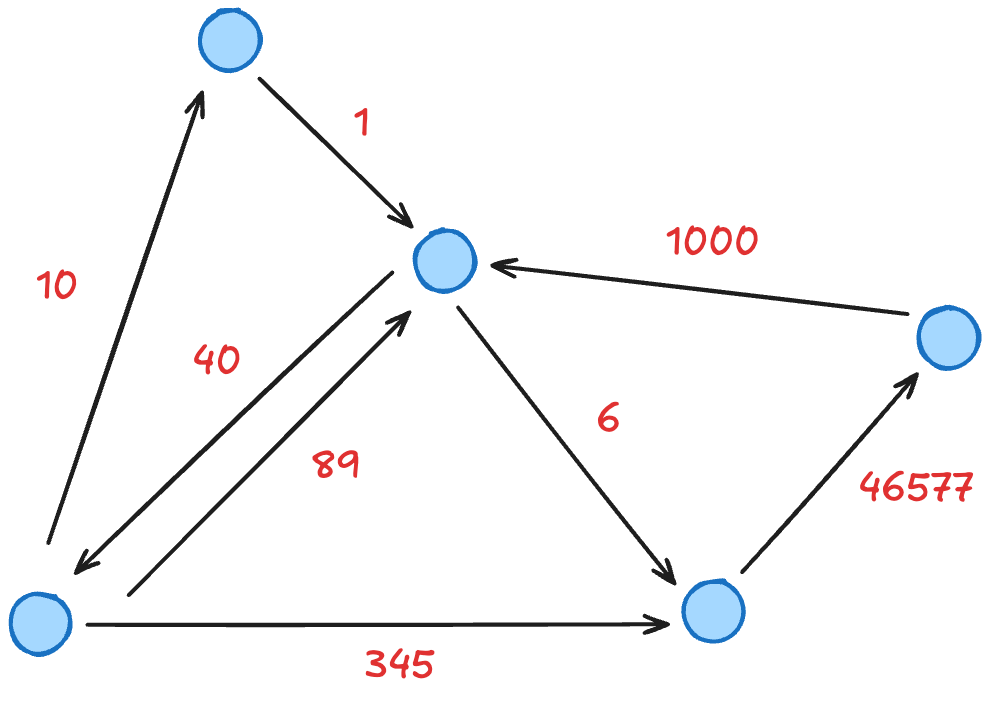
\includegraphics[width=0.85\linewidth]{figures/c3/graph}
  \caption{Mô hình hoá orderbook thành đồ thị có hướng có trọng số}
  \label{fig:matching-graph}
\end{figure}

\subsubsection*{Vòng lặp điều phối}

Hai thành phần cộng tác để chạy việc khớp lệnh định kỳ:

\paragraph{\texttt{MatchScheduler}} là một vòng lặp dựa trên
\texttt{setInterval} với chu kỳ mặc định 5\,s (cấu hình qua
\texttt{MATCH\_INTERVAL\_MS}). Cứ mỗi 5 giây, scheduler gom toàn bộ
intent đang sống thành một \emph{batch} và gọi
\texttt{MatchingService.runTick()} để tìm các chu trình bù trừ trên
batch đó; cửa sổ 5 giây là sự cân bằng giữa việc cho đủ thời gian để
nhiều intent đối ứng cùng tích luỹ trong cùng một batch (tăng khả
năng tạo cycle) và việc giữ độ trễ chấp nhận được cho người dùng. Vì
Node.js là single-threaded, một cờ boolean \texttt{isRunning} là đủ
để ngăn các tick chồng lên nhau khi một tick chưa kịp hoàn tất;
không cần mutex.

\paragraph{\texttt{MatchingService.runTick()}} thực thi một tick:

\begin{enumerate}
  \item \textbf{Hết hạn.} Quét \texttt{OrderStore}, đánh dấu các order
    có \texttt{deadline} đã trôi qua thành \texttt{EXPIRED} và xoá khỏi
    pair index.
  \item \textbf{Snapshot.} Lấy mảng các order còn hoạt động
    (\texttt{QUEUED} hoặc \texttt{PARTIAL}).
  \item \textbf{Build graph.} Chuyển snapshot thành tập cạnh và xác
    định số đỉnh.
  \item \textbf{Tìm chu trình.} Gọi
    \texttt{runAlgorithm($n$, edges, $x$)} — chính là thuật toán giảm
    chu trình mô tả ở phần sau.
  \item \textbf{Translate.} Dịch các chu trình bắt được thành các
    đối tượng \texttt{MatchResult}: cập nhật trạng thái mỗi order
    bị ảnh hưởng thành \texttt{MATCHED} (đã được match toàn bộ) hoặc
    \texttt{PARTIAL} (mới được match một phần).
  \item \textbf{Persist.} Append \texttt{MatchResult} vào nhật ký match
    của \texttt{OrderStore} (qua đó được mirror sang Postgres).
  \item \textbf{Hand-off.} Trả \texttt{TickStats} cho scheduler;
    scheduler chuyển danh sách \texttt{MatchResult} sang Orchestrator
    để thực thi on-chain.
\end{enumerate}

\subsubsection*{Thuật toán giảm chu trình (cycle-reduction)}

Cốt lõi thuật toán nằm ở bước 4: tìm các chu trình \emph{đáng để khớp}
trong $G$ và đồng thời cập nhật $G$ để phản ánh phần đã được tiêu thụ.
Về mặt lý thuyết, bài toán \emph{tối đa hoá tổng khối lượng được khớp}
trên một đồ thị bất kỳ là NP-hard nếu yêu cầu nghiệm tối ưu toàn cục.
Do hệ thống cần chạy thời gian thực với chu kỳ 5\,s, OceanLink chọn
một chiến lược tham lam dựa trên DFS với một ngưỡng chấp nhận được.

\paragraph{Tham số ngưỡng $x \in [0, 1]$.} Cấu hình qua
\texttt{MATCH\_THRESHOLD} (mặc định $0.3$). Một chu trình $C$ chỉ
được khớp nếu

\[
  \mathrm{ratio}(C) \;=\; \frac{\min_{e \in C} w(e)}{\max_{e \in C} w(e)} \;>\; x.
\]

Ý nghĩa: tỉ số $\mathrm{ratio}$ đo độ \emph{cân bằng} của chu trình.
Khi $\mathrm{ratio} = 1$, mọi cạnh có cùng trọng số, vòng được khớp
hoàn toàn. Khi $\mathrm{ratio}$ rất nhỏ, chu trình có một cạnh quá
yếu so với các cạnh còn lại — chỉ một phần rất nhỏ tài sản có thể
được khớp, phần còn dư phải xếp hàng tiếp; chi phí gas khi thực thi
sẽ không đủ bù lại lợi ích. Ngưỡng $x$ là cơ chế tránh khớp các chu
trình "lệch" như vậy.

\paragraph{Bộ khung DFS ba màu.} Việc tìm một chu trình bất kỳ trong
đồ thị có hướng được thực hiện bằng DFS với ba màu:

\begin{itemize}
  \item \textbf{trắng} (0): đỉnh chưa được duyệt.
  \item \textbf{xám} (1): đỉnh đang nằm trên ngăn xếp DFS hiện tại.
  \item \textbf{đen} (2): đỉnh đã duyệt xong, mọi hậu duệ đã được
    khám phá.
\end{itemize}

Khi DFS phát hiện một cạnh trỏ đến đỉnh \emph{xám} (back-edge), một
chu trình tồn tại. Thuật toán duy trì một ngăn xếp các cạnh đang ở
trên đường DFS hiện tại, từ đó tái dựng chu trình bằng cách trích
phần đuôi của ngăn xếp tính từ cạnh nối đến đỉnh xám đó.

\paragraph{Bước cập nhật.} Sau khi xác định được một chu trình $C$
với $\mathrm{ratio}(C) > x$, thuật toán thực hiện ba việc:

\begin{enumerate}
  \item \textbf{Snapshot.} Lưu lại bản sao bất biến của các cạnh
    trong $C$ kèm trọng số tại thời điểm khớp. Snapshot này là dữ
    liệu nguyên thuỷ để Orchestrator dựng lại các \texttt{SendAction}.
  \item \textbf{Loại cạnh tối thiểu.} Cạnh có trọng số $w_{\min} =
    \min_{e \in C} w(e)$ bị xoá khỏi đồ thị (intent tương ứng được
    đánh dấu \texttt{MATCHED}, đã sử dụng trọn).
  \item \textbf{Trừ trọng số.} Mọi cạnh khác trong $C$ bị giảm
    trọng số đi đúng $w_{\min}$ — phần "đã tiêu" trên các intent
    còn lại. Các intent đó chuyển sang \texttt{PARTIAL} với phần
    còn lại trong queue chờ tick sau.
\end{enumerate}

Sau bước cập nhật, đồ thị mới có ít hơn ít nhất một cạnh; thuật toán
lặp lại từ đầu — DFS lại trên đồ thị mới — cho đến khi không còn chu
trình nào hoặc chu trình tìm được không thoả ngưỡng.

\paragraph{Mã giả tổng quát.}

\begin{verbatim}
function runAlgorithm(n, edges, x):
    capturedCycles <- []
    repeat:
        C <- findOneCycle(n, edges)         // DFS three-colour
        if C is empty: break
        let w_min = min(edge.w for edge in C)
        let w_max = max(edge.w for edge in C)
        if w_min / w_max <= x: break
        capturedCycles.append( snapshotOf(C) )
        remove the edge of weight w_min from edges
        for each remaining edge e in C:
            e.w <- e.w - w_min
    return capturedCycles
\end{verbatim}

\paragraph{Đảm bảo dừng (termination).} Mỗi vòng lặp loại đúng một
cạnh khỏi đồ thị, do $|E|$ luôn giảm sau mỗi lần lặp thành công.
Thuật toán dừng tối đa sau $|E|$ vòng lặp, vì vậy độ phức tạp là
$O(|E| \cdot |V| \cdot |E|) = O(|V| \cdot |E|^2)$ — DFS có chi phí
$O(|V| + |E|)$ và được lặp tối đa $|E|$ lần. Trong thực tế $|V|$ rất
nhỏ (số chuỗi) và $|E|$ giới hạn bởi số intent đang sống, nên chi phí
là chấp nhận được.

\paragraph{Tham lam và không tối ưu.} Thuật toán không bảo đảm tìm
được chu trình tốt nhất theo bất kỳ tiêu chí nào (tổng khối lượng,
tổng phí incentive, độ dài chu trình ngắn nhất). Đây là sự đánh đổi
có chủ đích:

\begin{itemize}
  \item \emph{Đơn giản, dễ kiểm chứng}: thuật toán chỉ phụ thuộc vào
    DFS chuẩn và phép so sánh trọng số, dễ test và dễ debug.
  \item \emph{Latency thấp}: hoàn tất trong vài mili-giây ngay cả khi
    có hàng chục intent.
  \item \emph{Đảm bảo "an toàn về kinh tế"}: ngưỡng $x$ ngăn
    việc khớp các vòng quá lệch có chi phí gas cao so với lợi ích.
\end{itemize}

Việc nâng cấp lên thuật toán tối ưu (ví dụ negative-cycle Bellman-Ford
trên một biến đổi của đồ thị, hay LP relaxation) được liệt kê trong
phần Future Work.

\subsubsection*{Ví dụ minh hoạ}

Xét đồ thị bốn cạnh: $0 \to 1$ trọng số 10, $1 \to 0$ trọng số 2,
$1 \to 2$ trọng số 8, $2 \to 1$ trọng số 4 và $x = 0.1$:

\begin{enumerate}
  \item \textbf{Vòng lặp 1.} DFS tìm thấy chu trình $0 \to 1 \to 0$.
    $\mathrm{ratio} = 2/10 = 0.2 > 0.1$ $\rightarrow$ khớp. Snapshot
    $[(0\to1, 10), (1\to0, 2)]$ được lưu. Cạnh $1 \to 0$ bị xoá.
    Cạnh $0 \to 1$ giảm còn 8.
  \item \textbf{Vòng lặp 2.} DFS tìm thấy chu trình $1 \to 2 \to 1$.
    $\mathrm{ratio} = 4/8 = 0.5 > 0.1$ $\rightarrow$ khớp. Snapshot
    $[(1\to2, 8), (2\to1, 4)]$ được lưu. Cạnh $2 \to 1$ bị xoá.
    Cạnh $1 \to 2$ giảm còn 4.
  \item \textbf{Vòng lặp 3.} Đồ thị còn lại $\{0\to1(8),\ 1\to2(4)\}$
    là acyclic; thuật toán dừng.
\end{enumerate}

Kết quả: hai chu trình được khớp trong cùng một tick. Hành vi này được
phủ trong test \texttt{algorithm.test.ts} và là cơ sở để Orchestrator
gom thành các order consolidated trên cùng chuỗi.

\subsubsection*{Liên kết với incentive fee}

\texttt{IntentOrder} cho phép người dùng kèm trường \texttt{incentiveFee}
\emph{tuỳ chọn}. Trọng số của cạnh không phải là số USDC nguyên gốc mà
là \emph{số tiền hiệu dụng}:

\[
  w(e) = \mathrm{amount}(e) + \mathrm{incentiveFee}(e).
\]

Hệ quả: các intent có incentive fee cao có cạnh nặng hơn, nên có nhiều
khả năng nằm trong chu trình thoả ngưỡng và được khớp trước. Đây là
một cơ chế đấu giá ngầm cho thứ tự ưu tiên match — không cần một sổ
giá riêng.
